\section{Untersuchung von Akkumulatorzellen} 

Dieser Teilversuch beschäftigt sich mit der Untersuchung der Innenwiderstände und der Leistungsabgabe von Akkumulatorzellen.
Zur Betrachtung dieser wird ein einfacher Schaltkreis mit diesen und einem äußeren Widerstand herangezogen.
Es wird die anliegende Klemmspannung gemessen und in Abhängigkeit des Widerstands gesetzt. 
Mit Hilfe der Darstellung der Spannungsquelle als Reihenschaltung von einer idealen Quelle und einem Innenwiderstand, sowie den Kirchhoff'schen Regeln wird dann der letzterer bestimmt. 
Das Ziel des Versuches ist die Übereinstimmung der gemessenen Werte mit den ermittelten. 
Dies wird bestätigt, da die gemessene Leerlaufspannung von z.B. \SI{1,2+-0,2}{V} für eine einzelne Akkumulatorzelle mit dem ermittelten Wert von \SI{1,260+-0,194}{V} übereinstimmt. Auch die Werte für drei in Reihe bzw. parallel geschaltete Akkumulatorzellen stimmen mit den Erwartungen überein.
Auch der Zusammenhang der Widerstände für die maximale Leistung wird bestätigt.  

\subsection{Methoden}

\subsubsection{Aufbau}

Der Aufbau dieses Versuchs beschränkt sich auf einen simplen Schaltkreis, welcher zunächst nur aus einer Akkumulatorzelle und einem regulierbaren Widerstand $R_a$ besteht. 
Zusätzlich dazu ist ein Multimeter an die Akkumulatorzelle geschlossen, sodass die dort anliegende Spannung gemessen werden kann. 
Mit diesem Aufbau wird zuerst die Leerlaufspannung $U_0$ der Akkumulatorzelle und dann der Innenwiderstand $R_i$ dieser bestimmt.
Dazu wird die Klemmspannung $U_{kl}$ gemessen und in Abhängigkeit des elektrischen Stroms $I$ gesetzt, welcher sich durch die Spannung und dem anliegenden Widerstand bestimmen lässt.

Dieser Vorgang wird dann für drei in Reihe- und drei parallel geschaltete Akkumulatorzellen wiederholt. 

\subsubsection{Unsicherheiten}

Bei diesem Versuch treten lediglich die Unsicherheit des Multimeters und des Lastwiderstands $R_a$ auf. 
Da das Multimeter eine analoge Darstellung der Messwerte verwendet und sich je nach verwendeter Größenordnung mit einer Genauigkeit von \SI{1}{V} bzw. \SI{0,1}{V} ablesen ließ, werden die zugehörigen Unsicherheiten über eine Dreiecksverteilung bestimmt.
Für die Unsicherheit des Widerstands wird, da es sich hierbei um einen alten Stöpselwiderstand, eine prozentuale Abweichung des angegebenen Werts von 10\% gewählt.
Im Allgemeinen werden zur Berechnung der kombinierten Unsicherheiten die nach GUM vorgesehenen Formeln verwendet. 
Die Berechnung dieser für diesen Versuch erfolgt im Anhang (\ref*{sec:anhang}).

\subsection{Datenanalyse}

Alle aufgenommenen Werte sind dem Laborbuch zu entnehmen. 
Darüber hinaus sind die Daten in den folgenden Diagrammen graphisch dargestellt.
\begin{figure}[ht]
	\centering
	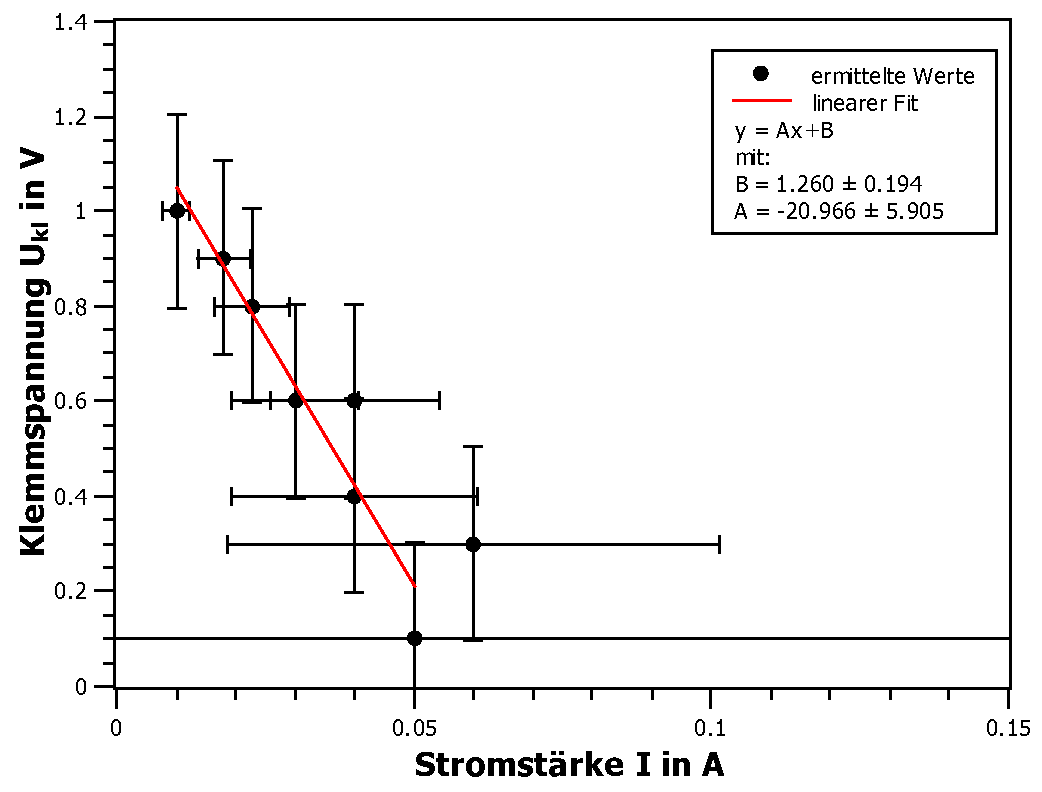
\includegraphics[width=0.9\textwidth]{auswertung/I-U1.pdf}
	\caption{Graphische Darstellung der Klemmspannung $U_{kl}$ in Abhängigkeit des elektrischen Stroms $I$ im Falle einer einzelnen Akkumulatorzelle. Der Betrag der Steigung des linearen Fits stellt den Innenwiderstand $R_i$ dar.}
	\label{fig:IU1}	
\end{figure}
\begin{figure}[ht]
	\centering
	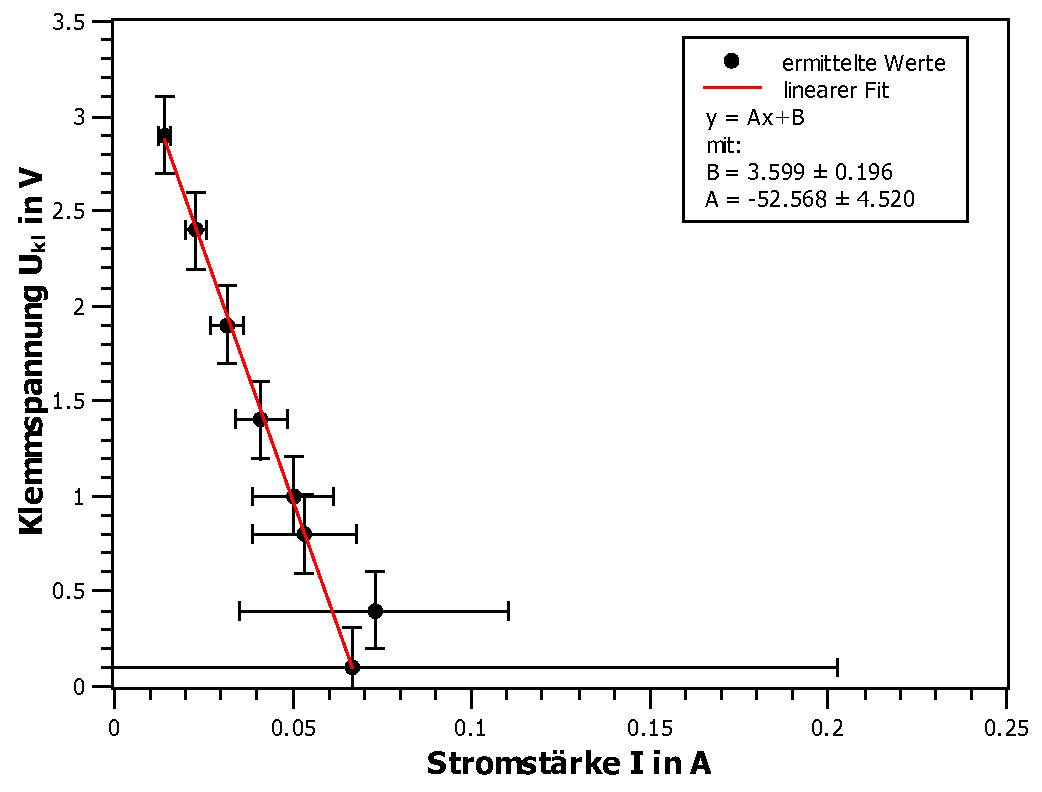
\includegraphics[width=0.9\textwidth]{auswertung/I-U2.pdf}
	\caption{Graphische Darstellung der Klemmspannung $U_{kl}$ in Abhängigkeit des elektrischen Stroms $I$ im Falle von drei in Reihe geschalteten Akkumulatorzellen. Der Betrag der Steigung des linearen Fits stellt den Innenwiderstand $R_i$ dar.}
	\label{fig:IU2}	
\end{figure}
\begin{figure}[ht]
	\centering
	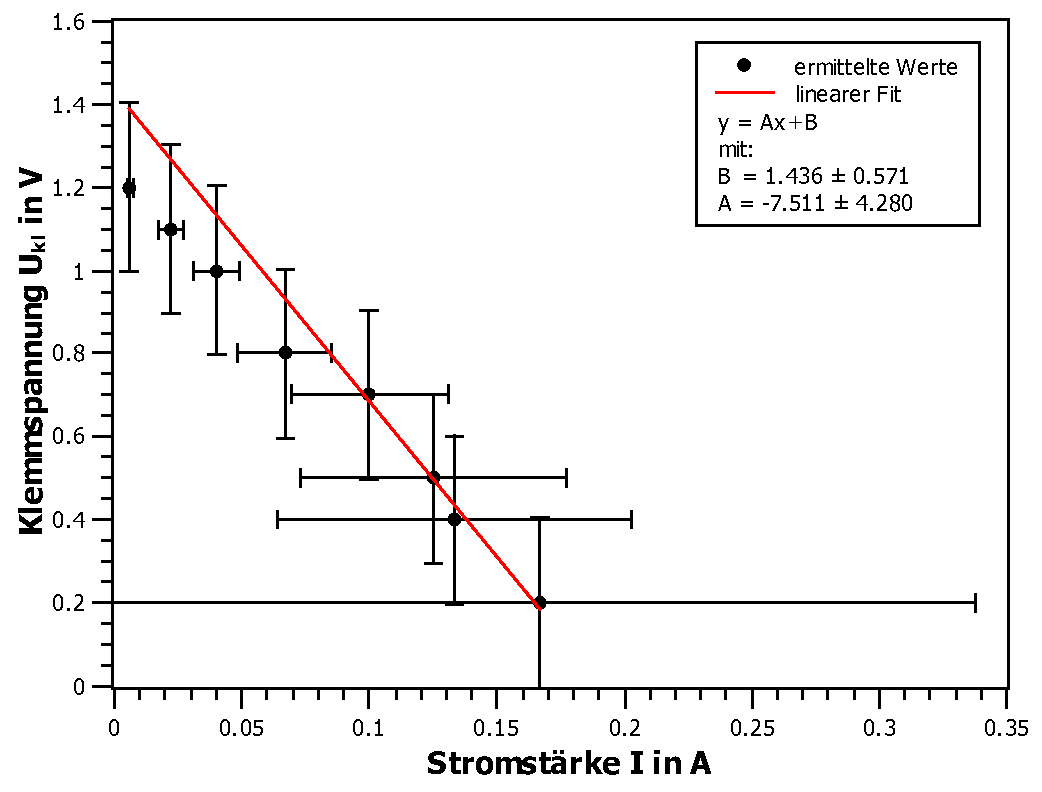
\includegraphics[width=0.9\textwidth]{auswertung/I-U3.pdf}
	\caption{Graphische Darstellung der Klemmspannung $U_{kl}$ in Abhängigkeit des elektrischen Stroms $I$ im Falle von drei parallel geschalteten Akkumulatorzellen. Der Betrag der Steigung des linearen Fits stellt den Innenwiderstand $R_i$ dar.}
	\label{fig:IU3}	
\end{figure}
\begin{figure}[ht]
	\centering
	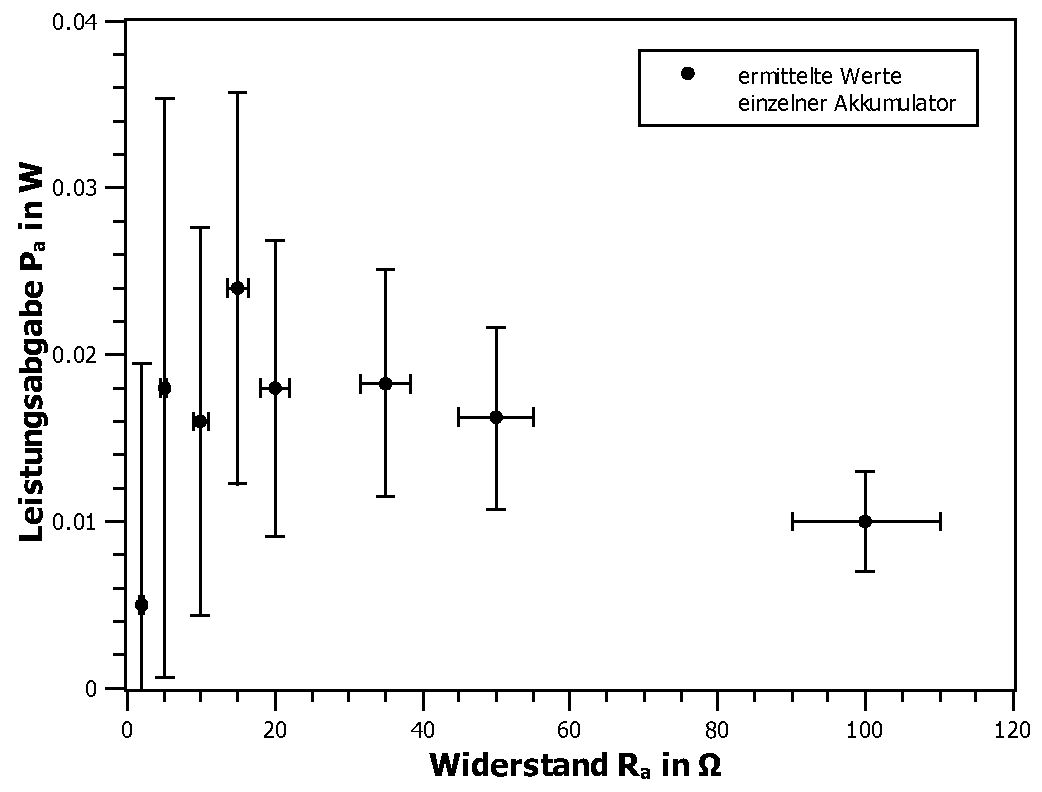
\includegraphics[width=0.9\textwidth]{auswertung/R-P1.pdf}
	\caption{Graphische Darstellung der Leistungsabgabe $P_a$ in Abhängigkeit des Außenwiderstands $R_a$ im Falle einer einzelnen Akkumulatorzelle. Das Maximum liegt nahe des Innenwiderstands von \SI{20,966+-5,905}{\Omega}.}
	\label{fig:RP1}	
\end{figure}
\begin{figure}[ht]
	\centering
	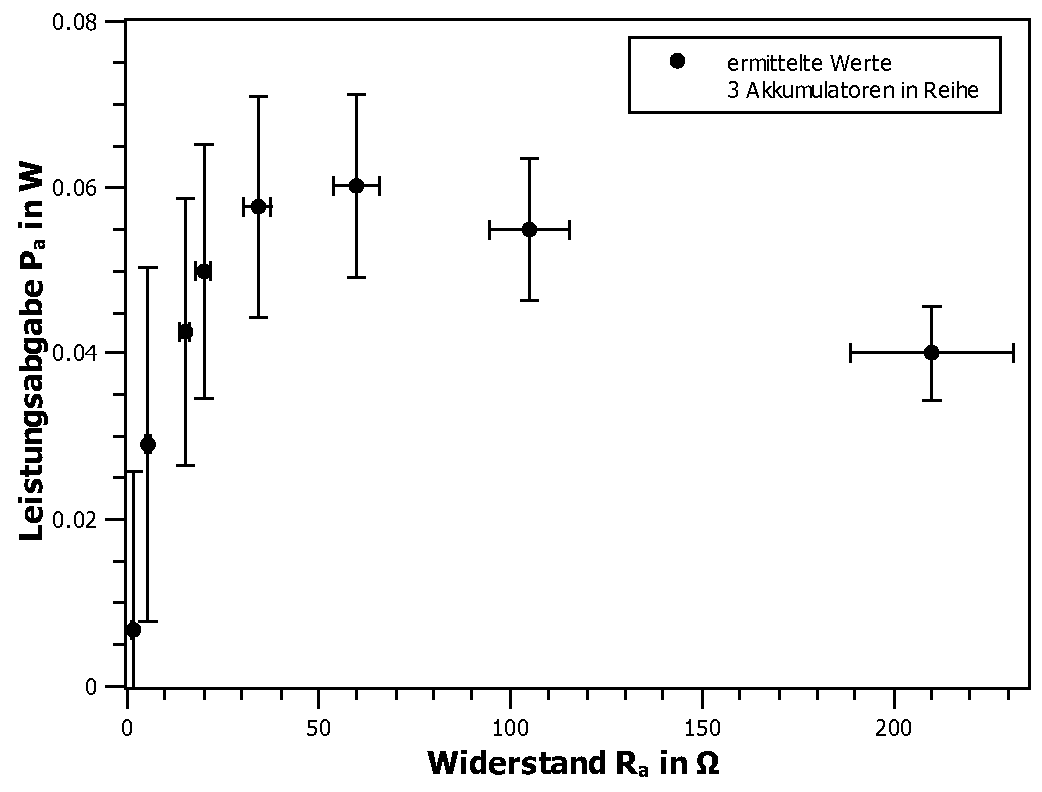
\includegraphics[width=0.9\textwidth]{auswertung/R-P2.pdf}
	\caption{Graphische Darstellung der Leistungsabgabe $P_a$ in Abhängigkeit des Außenwiderstands $R_a$ im Falle von drei in Reihe geschalteten Akkumulatorzellen. Das Maximum liegt nahe des Innenwiderstands von \SI{52,568+-4,520}{\Omega}.}
	\label{fig:RP2}	
\end{figure}
\begin{figure}[ht]
	\centering
	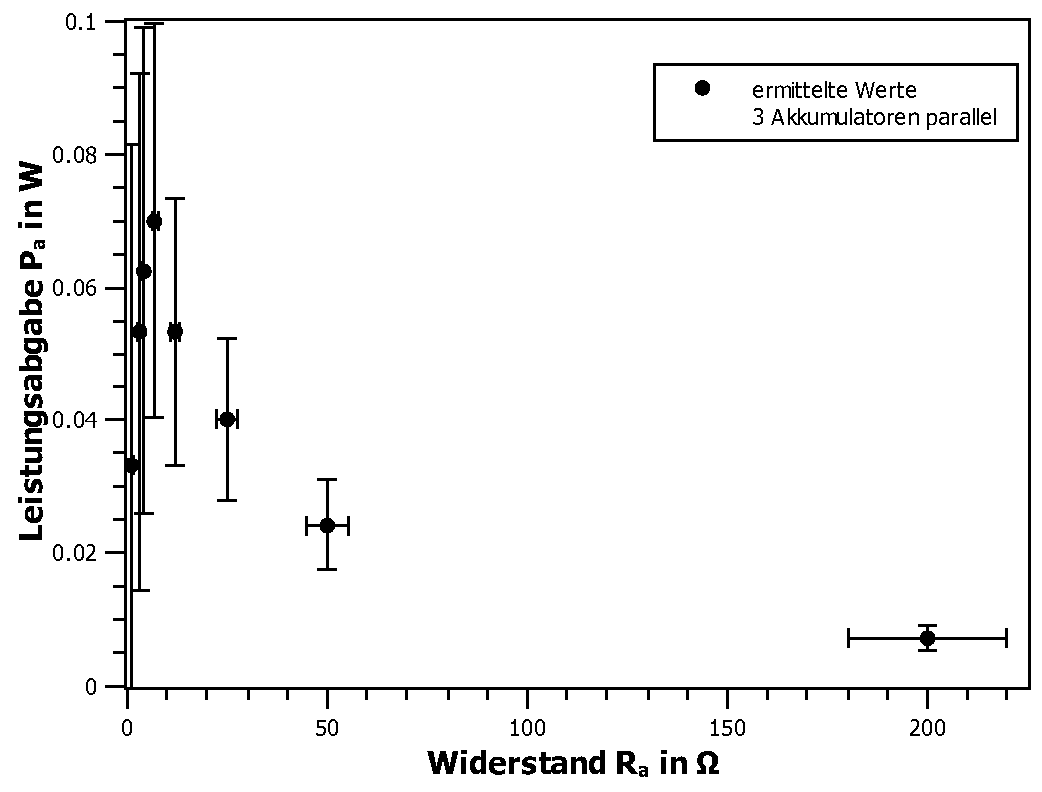
\includegraphics[width=0.9\textwidth]{auswertung/R-P3.pdf}
	\caption{Graphische Darstellung der Leistungsabgabe $P_a$ in Abhängigkeit des Außenwiderstands $R_a$ im Falle von drei parallel geschalteten Akkumulatorzellen. Das Maximum liegt nahe des Innenwiderstands von \SI{7,511+-4,280}{\Omega}.}
	\label{fig:RP3}	
\end{figure}

Zur Bestimmung der Leerlaufspannung wird ein "unendlich" großer Widerstand gewählt, der Stromkreis ist also nicht geschlossen.
Für diese ergeben sich \SI{1,2+-0,2}{V} für die einzelne Akkumulatorzelle, \SI{3,7+-0,2}{V} drei in Reihe geschaltete Zellen und erneut \SI{1,2+-0,2}{V} drei parallel geschaltete Akkumulatorzellen. 

Da es sich bei der Akkumulatorzelle um keine ideale Spannungsquelle hält, was sich physikalisch auch nicht realisieren lässt, wird sie als Reihenschaltung von idealer Spannungsquelle $U_0$ und Innenwiderstand $R_i$ angenommen. 
Nach dem zweiten Kirchhoff'schen Gesetz folgt mit Belastung eines äußeren Widerstands:
\begin{align}
	U_0 = R_i I + R_a I \\
	\text{und durch umformen nach $R_i$ folgt:} \quad R_i = \frac{U_0}{I}-R_a.
\end{align}
Der elektrische Strom $I$ lässt sich hierbei durch die gemessene Klemmspannung $U_{kl}$ und dem Widerstand $R_a$ ermitteln ($I=\frac{U_{kl}}{R_a}$).
Zu Beachten ist hierbei, dass sich kein Wert für einen Außenwiderstand von \SI{0}{\Omega} ermitteln lässt, da dafür durch null geteilt werden müsste.
In diesem Falle kommt es zum Kurzschluss.
Dabei ist der Strom maximal, aber endlich, kann jedoch zur Rechnung nicht verwendet werden.
Ebenso führt die oben angegebene Formel für einen unendlich großen Außenwiderstand dazu, dass der Innenwiderstand gegen null geht, da sich $U_{kl}$ der Leerlaufspannung $U_0$ annähert und $R_i = R_a - R_a = 0$ übrig bleibt.
Umformen der oberen Gleichung nach der Klemmspannung $U_{kl} = R_a I$ lässt darauf schließen, dass der Innenwiderstand $R_i$ sich auch als Steigung der Gleichung $U_{kl} = -R_i I + U_0$ identifizieren lässt. Dies ist in den Diagrammen \ref{fig:IU1} bis \ref{fig:IU3} für die drei Fälle dargestellt\footnote{Die Fits und deren Unsicherheiten wurden von dem Programm SciDavis berechnet, dazu wurden die Unsicherheiten (welche im Anhang zu finden sind) und die Methode der kleinsten Quadrate herangezogen}.
Somit ergibt sich ein Innenwiderstand von \SI{20,966+-5,905}{\Omega} für eine einzelne Akkumulatorzelle, \SI{52,568+-4,520}{\Omega} für drei in Reihe geschaltete Zellen und \SI{7,511+-4,280}{\Omega} für drei parallel geschaltete Akkumulatorzellen. 
Daraus folgt, dass sich der Innenwiderstand in einer Größenordnung von einem zwei-stelligen \si{\Omega}-Bereich befindet. 

Nun zu der Betrachtung der Leistungsabgabe.
Diese setzt sich zunächst allgemein aus $P = UI$ zusammen. 
Dabei sind hier $U = U_{kl}$ und $P=P_a$.
Umformen führt zu
\begin{equation}
	P_a = U_0^2\frac{R_a}{(R_a+R_i)^2}
\end{equation}
In Abhängigkeit des Innenwiderstands ist die Leistungsabgabe für $R_a = R_i$ maximal (gilt nur für ohm'sche Widerstände). 
Die Leistungsanpassung geschieht durch die Annäherung der Widerstände, sodass die Leistung des Verbrauchers maximal ist, dies ist gerade bei $P_{max} = \frac{U_0^2}{4R_i}$ der Fall.

Für die drei Fälle ist $P_a$ in Abhängigkeit des Außenwiderstands $R_a$ in den Diagrammen \ref{fig:RP1} bis \ref{fig:RP3} dargestellt. 
Da nur wenige Messpunkte vorliegen, ist der genaue Wert für $R_a$ bei dem die Leistung maximal ist nicht genau zu erkennen.
Jedoch fällt auf, dass die Punkte, welche am höchsten liegen alle nahe von einer Standardunsicherheit der oben aufgeführten Innenwiderstände, für den jeweiligen Fall, liegen.

\subsection{Diskussion}

Vergleicht man nun die Messergebnisse, so fällt auf, dass diese mit den zu erwartenden übereinstimmt. 
Der Y-Achsenabschnitt bei den $I$-$U$-Diagrammen stellt nach den Gesetzen von Kirchhoff die Leerlaufspannung dar.
Die gemessenen Werte liegen alle innerhalb einer Standardunsicherheit der durch den Fit ermittelten Werte.
Um einen konstanten Strom zu erhalten, sollte der Innenwiderstand möglichst hoch gewählt werden, also eine Reihenschaltung von gleichen Spannungsquellen sollte dazu verwendet werden.
Für eine konstante Spannung hingegen sollte ein möglichst geringer Innenwiderstand gewählt werden, was durch eine Parallelschaltung von gleichen Spannungsquellen erreicht werden kann.
Auch das Verhältnis für die maximale Leistung ($R_a = R_i$) kann aus den Diagrammen, trotz großer Ungenauigkeiten, entnommen werden.
Eine genauere Aufnahme der Werte wäre an dieser Stelle sinnvoll.

\subsection{Schlussfolgerung}

Das Ziel, eine Bestätigung der verwendeten Theorie, wurde erreicht. 
Dies gilt für die zweite Kirchhoff'sche Regel, sowie dem Zusammenhang der Leistung, der Spannung und der Stromstärke.
Aufgrund der großen Unsicherheiten, scheint es sinnvoll den Versuch zu wiederholen, wobei deutlich mehr Werte aufgenommen werden sollten, sodass die graphische Auswertung für die Leistungsabgabe eindeutiger wird und kleinere Unsicherheiten angenommen werden können.
Zu den großen Unsicherheiten trägt hauptsächlich die des Widerstands bei, da 10\% von großen Widerständen hierbei nicht wenig sind.
Da die meisten Werte auch mit deutlich kleineren Unsicherheiten im Erwartungsbereich liegen würden, kann die Größe dieser für das Fazit weniger stark berücksichtigt werden.
